% Frugal AI seminar, part 6: efforts you can reproduce. All numbers here were run by us; device and date are
% stated. The Gemma results use stub weather data and temperature 0 (replies were identical across tries).
% CheatSheet-safe: no floats, the table is wrapped in adjustbox.

\section[Efforts]{Efforts You Can Reproduce}

%%%%%%%%%%%%%%%%%%%%%%%%%%%%%%%%%%%%%%%%%%%%%%%%%%%
\begin{frame}[fragile]\frametitle{}
\begin{center}
{\Large Efforts You Can Reproduce}

\medskip
{\small (Code, numbers and honest limits)}
\end{center}
\end{frame}

%%%%%%%%%%%%%%%%%%%%%%%%%%%%%%%%%%%%%%%%%%%%%%%%%%%
\begin{frame}[fragile]\frametitle{An Offline Wiki on an Old Laptop}
\begin{itemize}
\item Ask questions of a folder of markdown notes. Retrieval is BM25 in pure Python (no model, no extra packages); embeddings are an option; a small local model answers only from the retrieved notes and names the note it used.
\item Arithmetic goes to a safe calculator and never reaches the model.
\item Measured on a small made-up sample wiki: the right note ranked first for 10 of 10 questions, with BM25 alone and with embeddings added; retrieval takes under 1 ms.
\item Honest limit: the sample is small and easy. It shows the pipeline works, not how it performs on your real notes.
\end{itemize}
{\tiny (Ref: FrugalAI repository, recipes/offline-wiki-rag, 19 October 2026)}
\end{frame}

%%%%%%%%%%%%%%%%%%%%%%%%%%%%%%%%%%%%%%%%%%%%%%%%%%%
\begin{frame}[fragile]\frametitle{AIOOLL: AI on an Old Linux Laptop}
\begin{itemize}
\item Six independent modules, each with a runnable driver, tests and a Streamlit UI: classical ML, deep learning, RAG, agents, computer vision, local LLM inference.
\item Local models through Ollama; the README lists Gemma 2 2B, Qwen2 1.5B, TinyLlama 1.1B, Phi-3 Mini 3.8B and an embedding model.
\item Offline by design: no module may need the internet at run time.
\item Open source (MIT), and the first entry in the FrugalAI awesome list.
\end{itemize}
{\tiny (Ref: github.com/yogeshhk/AIOOLL)}
\end{frame}

%%%%%%%%%%%%%%%%%%%%%%%%%%%%%%%%%%%%%%%%%%%%%%%%%%%
\begin{frame}[fragile]\frametitle{One Small Model, Five Designs}
\begin{center}
\adjustbox{max width=0.95\linewidth, max totalheight=0.17\textheight}{%
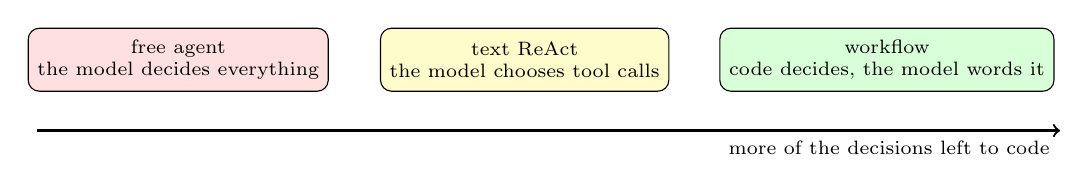
\begin{tikzpicture}
\tikzstyle{b}=[draw, rounded corners, align=center, minimum height=0.8cm, font=\scriptsize]
\node[b, fill=red!12, minimum width=3.4cm] (a) at (0,0) {free agent\\the model decides everything};
\node[b, fill=yellow!20, minimum width=3.4cm] (w) at (4.4,0) {text ReAct\\the model chooses tool calls};
\node[b, fill=green!15, minimum width=3.8cm] (c) at (9.0,0) {workflow\\code decides, the model words it};
\draw[->, thick] (-1.8,-0.9) -- (11.2,-0.9) node[below left, font=\scriptsize] {more of the decisions left to code};
\end{tikzpicture}}
\end{center}
\begin{itemize}
\item Task: weather questions with a weather tool, \texttt{gemma-2-2b-it} (Q4\_K\_M) in LM Studio, temperature 0, stub weather data. ``Text ReAct'': the model writes an Action line as plain text and our code runs the tool.
\end{itemize}
\begin{center}
\scriptsize
\adjustbox{max width=\linewidth}{%
\begin{tabular}{p{0.46\linewidth}p{0.50\linewidth}}
\hline
Design & What happened \\
\hline
Agent with built-in tool calling & Tool called in 0 of 5 tries; the model answered in plain text instead \\
Text ReAct, one-city question & Correct in 6 of 6 tries \\
Text ReAct, two-city question & Failed 3 of 3: it guessed a final answer in the same reply as the action, forgot a result and hit the step limit; one guess was wrong \\
Workflow, the model compares two numbers & Wrong 5 of 5: ``10.2 is higher than 11.4'' \\
Workflow, code compares, the model words the result & Right direction 5 of 5 (but its sentence dropped the number) \\
\hline
\end{tabular}}
\end{center}
\begin{itemize}
\item Lesson: use code for what code does well (compare, route, validate) and the model for language.
\end{itemize}
{\tiny (Ref: our runs, 19 October 2026; one model, one machine, small samples)}
\end{frame}

%%%%%%%%%%%%%%%%%%%%%%%%%%%%%%%%%%%%%%%%%%%%%%%%%%%
\begin{frame}[fragile]\frametitle{The Awesome List}
\begin{itemize}
\item \textbf{AWESOME.md} in the FrugalAI repository: a curated list of frugal AI efforts, one section per platform (old laptop, Raspberry Pi, phones, microcontrollers, browser) plus models, tools, applications, benchmarks and learning.
\item \textbf{Criteria}: free to use and open to all, a downloadable model, no per-token charges, and a statement of the hardware it was run on.
\item \textbf{To add yours}: an issue form or a pull request, then a small script checks the format.
\item Each entry carries a ``verified'' date, so the list stays honest as tools change.
\end{itemize}
\end{frame}
